\pdfbookmark{Parallelization Approaches}{parallelization approaches}
\chapter{Parallelization Approaches}
\label{ParallelizationApproaches}

As presented in chapter \ref{Application}, the critical region of the \tth application is the \ttDilepKinFit, which its execution time increases linearly with the number of variations per combination. With the initial optimizations already applied to the original application, presented in section \ref{InitialOptimizations}, the next step is to resort to parallelization. This chapter presents four parallelization approaches, two on homogeneous systems and two on heterogeneous systems, one using GPU and other using \intel Xeon Phi as hardware accelerators.

Although the critical region is the \ttDilepKinFit function, the best parallelization strategy is to simultaneously perform the reconstruction of different events. All event processing is data independent so no synchronizations are necessary, reducing the parallelization overhead. Figure \ref{fig:EventParallelization} presents a schematic representation of this parallelization approach. However, as explained in section \ref{Application:Flow}, all the event data is stored globally to the application and partially in the LipMiniAnalysis library. Every time an event is loaded the global data is overwritten, which, in a parallel shared memory environment, causes the intermidiate results of the event processing of one thread to be overwritten by the processing of other thread.

\begin{figure}[!htp]
	\begin{center}
		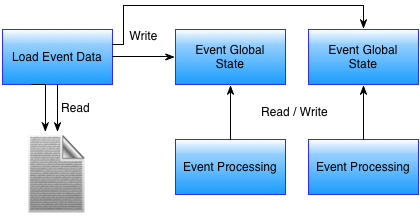
\includegraphics[scale=0.7]{../../common/img/2global_states_par.png}
		\caption{Schematic representation of the event-level parallelization model.}
		\label{fig:EventParallelization}
	\end{center}
\end{figure}

Each input file has around 1 GByte that makes possible to store all events on RAM memory. The use of a proper data structure for storing the event information would benefit the application structure and allow the possibility of this parallelization approach. In the current implementation the event are loaded before the processing. The application would benefit from the sequential read performance of hard drives, compensating the overhead of the data structure creation. The complexity of the changes necessary to both the application source code and LipMiniAnalysis library render this approach unreliable for the timeframe of this thesis dissertation.

The \ttDilepKinFit function mostly handles with data in its scope. The global data modified by this function can be managed without any modifications in the LipMiniAnalysis. Looking at the information presented in section \ref{ComputationalCharactrization}, specifically in figure \ref{fig:KinFitGraph}, can be expected that most performance gains can occur for 16 to 512 variations per combination as \ttDilepKinFit occupies most of the application execution time, rather that for a smaller number of variations.

The \ttDilepKinFit execution is irregular, meaning that dependent on the event to be reconstructed its execution time varies. This is caused by the number of Bottom Quark jets and leptons combinations, which is different for each event. Also, it is dependent on the kinematical reconstruction. If the \ttbar system is possible to reconstruct, \ttDilepKinFit attempts to reconstruct the Higgs Boson. If not, the Higgs Boson is not reconstructed, reducing the function execution time. This translates in an irregular workload much more likely to affect the performance if the load balancing strategy is not suited for the problem.

The kinematical reconstruction is performed in the \dilep function. The \ttbar system obeys a set of properties expected from the Top Quark theoretical model. To reconstruct both of the Top Quarks it is needed to know the characteristics of all resultant particles from their decay. However, since the neutrinos do not react with the detector, and their characteristics are not recorded, it is needed to infer them, using various properties, such as momentum and energy conservation of the system. Once the neutrinos characteristics are determined, it is possible to reconstruct the Top Quarks. \dilep analitically solves a system of 6 equations to infer the neutrinos characteristics and then reconstruct the Top Quarks. The function is dependent on only one class from ROOT, TLorentzVector, making it easy to port to GPU. Also, it is the function that only handles data private to the function.

\pdfbookmark{Shared Memory Parallelization}{shared memory parallelization}
\section{Shared Memory Parallelization}
\label{Parallelization:SharedMem}

Figure \ref{fig:SeqPipeline} (left) illustrates the workflow of the \ttDilepKinFit. The best approach is to parallelize the loop that iterates through all the jets/leptons combinations. However, the computation of the combinations cannot be performed in parallel as for chosing one combination it is necessary to know every combinations chosen so far. Also, the combinations information is stored globally to the application so a data structure must be created to allow parallel reconstructions of different combinations.

\begin{figure}[!htp]
	\begin{center}
		\raisebox{-0.5\height}{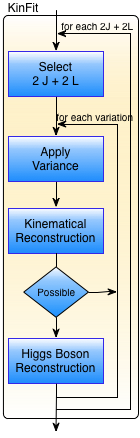
\includegraphics[scale=0.7]{../../common/img/sequential_kinfit.png}}
		\raisebox{-0.5\height}{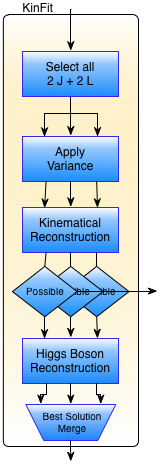
\includegraphics[scale=0.7]{../../common/img/parallel_kinfit.png}}
		\caption{Schematic representation of the \ttDilepKinFit sequential (left) and parallel (right) workflows.}
		\label{fig:SeqPipeline}
	\end{center}
\end{figure}

The number of parallel tasks will be equal to the number of total reconstructions to process, which is the number of combinations times the number of variations per combination. This small granularity allows for the scheduler responsible for the load balance to better distrubute the work among the threads used. Each task has a combination assigned and it applies a variation and reconstructs it. The result is stored in a state private to the task so that, after all variations of all combinations are computed, only the best solution is considered, performed by a reduction. The reduction can also be parallelized, reducing its complexity from \textit{O(N)} to \textit{O($log_{2}$(N))}, where \textit{N} is the number of elements to reduce.

\begin{figure}[!htp]
	\begin{center}
		\raisebox{-0.5\height}{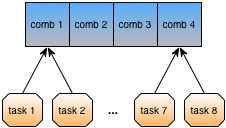
\includegraphics[scale=0.7]{../../common/img/parallel_methodology.png}}
		\raisebox{-0.5\height}{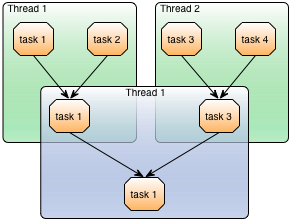
\includegraphics[scale=0.7]{../../common/img/parallel_reduction.png}}
		\caption{Schematic representation of the parallel tasks accessing the shared data structure (left) and the new parallel reduction (right).}
		\label{fig:ParallelMethodology}
	\end{center}
\end{figure}

Figure \ref{fig:ParallelMethodology} presents the parallelization strategy using concurrent tasks sharing the combinations data structure and the strategy for the parallel reduction. This modifications to the workflow are schematized in figure \ref{fig:SeqPipeline} (right). As stated before, chosing the combinations and building the data structure cannot be performed in parallel. This reduces the parallelizable region and adds an extra overhead to each \ttDilepKinFit call. Also, the best solution merge, which does not happens in the sequential application, increases this overhead. This process is repeated for each event.

\subsection{Implementation}
\label{SharedMemImplementation}

The implementation was performed iteratively, where every major change impact is tested in terms of performance and correctness of the application output before proceeding to the next change. Since the application code is very complex has a big global state, small modifications, specially when introducing parallelism, can completly alter the application behavior. OpenMP library was used to implement the parallelization as it is the most used among scientists and easier to include in C-like applications such as \tth. It offers many functionalities required by the parallelization strategy, such as parallel reductions, various workload schedulers and explicit thread management and synchronization primitives. Also, OpenMP allows for the number of threads to be defined by environment variables, without any changes to the code.

Each step of the \ttDilepKinFit workflow (see figure \ref{fig:SeqPipeline}, left image) was individually parallelized to control the impact of the concurrent tasks on the overall behavior. Then, all the parallel regions were concatenated, resulting in the workflow presented in figure \ref{fig:SeqPipeline}, right image. At this point the application performance was not a concern.

The first task performed by \ttDilepKinFit is chosing the variations. This can be performed while building the data structure holding its information, and must be a serial process since chosing a combination depends on all previous choices. The total amount of combinations, which depends on the amount of jets and leptons $n$, pairing two jets with two leptons, being $k = 4$, in the same combination regardless of their order, i.e. $(j_1, j_2) = (j_2, j_1)$, is, according to the formula for mathematical combinations, presented in equation \ref{eq:Combination}. The average number of combinations for the input data file is XX.

\begin{center}
	\begin{equation}
		\binom{n}{k} = \frac{n!}{k!(n - k)!} \mbox{, with k = 4 then } \binom{n}{4} = \frac{n!}{8(n - 4)!}
		\label{eq:Combination}
	\end{equation}
\end{center}


All the information of the Bottom Quark jets and leptons (ROOT \texttt{TLorentzVector} class instances), as well as other control and auxiliary information is stored in a class built for this purpose. The function responsible for the variation of the parameters was implemented as a method of this class, increasing the modularity of the code. Each task creates a local copy of the combination to apply the variation and reconstruct. This keeps the integrity of the original combination parameters allowing it to be varied any number of times. Otherwise, applying a variation to an already varied combination would result in inaccurate physics results.

The size of one data structure element is 2 kB, and, on average, each event has 131 combinations, making the average data structure size 262 kB per event. Even though the data structure size is not big, the overhead of its construction might prove to be a factor limiting the performance. Note that the number of variations does not affect the size of the data structure.

One of the major problems of the parallelization is controlling the access to the global state. In \ttDilepKinFit, 34 global variables of mostly ROOT classes instances and vectors, are read and write inside the parallel region. The access to this variables can be serialized but that would alter the behavior of concurrent tasks reconstructing different variations of the same combination. Further analysis of the source code reveals that even though these variables are global they are only modified by the \ttDilepKinFit function to store intermidiate results. The most efficient solution is to create a local copy of the global state in each thread (note that a thread contains one or more parallel tasks), so that the parallel tasks do not have any data dependencies, avoiding serial accesses to shared resources that can cause contention and degrade the performance.

Only the best solution is needed after reconstructing all variations of all combinations for an event. The best solution, i.e., information resultant from the event reconstruction, can be measured by computing its quality. The result is a scalar value and the higher the value the better the reconstruction. The best solution is a set of 16 LipMiniAnalysis \texttt{TLorentzVectorWFlags}, an extension to the ROOT \texttt{TLorentzVector} class, and the scalar with the solution quality. To increase the modularity of the code a class was created that holds all this information and implements all comparator operations. This increases the implementation overhead but reduces the complexity of the reduction process. Since OpenMP only supports parallel reduction for scalars, a custom parallel reduction was implemented. The reduction is not performed among all tasks but rather among the threads used; during the reconstructions, each thread automatically holds the information of only the best solution which is then used in the reduction, diminishing the amount of elements to compare in the parallel reduction. After the reduction, the best solution information is copied to the global state.

The algorithm used for the reduction is simple. The threads are grouped two by two in each level of the reduction tree and they compare their solutions. The thread with the lower id keeps the best solution of the two. Threads which do not have a pair check a queue of threads with no pairs, and pick a pair. They are put in the queue if it is empty. An example reduction is presented in figure \ref{fig:Reduction}.

\begin{figure}[!htp]
	\begin{center}
		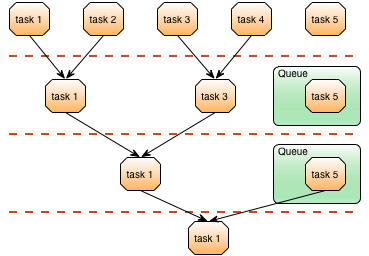
\includegraphics[scale=0.7]{../../common/img/parallel_reduction_example.png}
		\caption{Schematic representation of the event-level parallelization model.}
		\label{fig:Reduction}
	\end{center}
\end{figure}

As mentioned in section \ref{InitialOptimizations}, the random number generator used for applying the variations is the \texttt{TRandom3} ROOT class. It uses the Mersenne Twister algorithm which heavily depends on a huge global state. Concurrent threads cannot use the same global state because one thread random number generation would influence the other thread generation and they would have to be serialized. However, it is perfectly possible that different threads use different global states, eliminating the resource contention and correlations between random numbers. In this implementation, each thread has its own instance of the \texttt{Trandom3} class, ensuring that there are no global states shared and allowing for thread safe pseudo-random number generation.

OpenMP offers a set of different schedulers from which the most relevant are the static and dynamic schedulers. The static scheduler defines the number of parallel tasks that each thread will process prior to its execution. This scheduler requires a small amount of execution time and is very efficient for balancing regular workloads. For irregular workloads, such as \ttDilepKinFit, the static scheduler porduces a poor workload balance, which can affect the performance. The dynamic scheduler requires more computational power but performs a better job at balancing irregular workloads. The scheduler monitors the execution load of each thread and maps the tasks to the threads at runtime. Parallel implementations performance using both schedulers are analyzed and compared in subsection \ref{SharedMemPerformance}.

\todo{Isto do vtune aqui???}

\intel VTune tool was used to analyze and identify the bottlenecks of the parallel implementation. With the help of VTune, the constructor of the data structure was identified as the main performance bottleneck. When analyzing the data structure source code, as well as \ttDilepKinFit, its evident that some of its parameters are only read and not modified during each event processing. Instead of copying these parameters in each data structure element a it is possible to use pointer to their memory position in the global state. The access to this data can be parallel as it is read-only. However, it may decrease the performance when using two CPUs, as threads in one CPU may have to access data in other CPU, instead of holding a copy of the information in cache, which is possible when not using pointers. The performance of this implementation, which will be addressed as pointer version, is compared against the previous implementation in subsection \ref{SharedMemPerformance}.

\subsection{Performance Analysis}
\label{SharedMemPerformance}

The performance analysis of the various shared memory implementations will be presented in this section. Many metrics of evaluating performance will be used, such as speedup and throughput, and the results will be analyzed and discussed. In this section the test system used is the compute-711 node if no other information is given.

Figures \ref{fig:RegularSpeedup} and \ref{fig:PointerSpeedup} present the speedups for various number of threads, using one and two CPUs with and without Multithreading\footnote{Refer to appendices \ref{App:TestEnv} and \ref{App:TestMethodology} for test system and methodology characterization.}. The maximum theoretical speedup is also presented in figure \ref{fig:AmdahlSpeedup} to compare the efficiency of the parallelization with the already optimized original sequential application. It is expected that the overhead of creating the data structure and merging the results may affect slightly the performance, specially for a small number of variations.

\begin{figure}[!htp]
	\begin{center}
		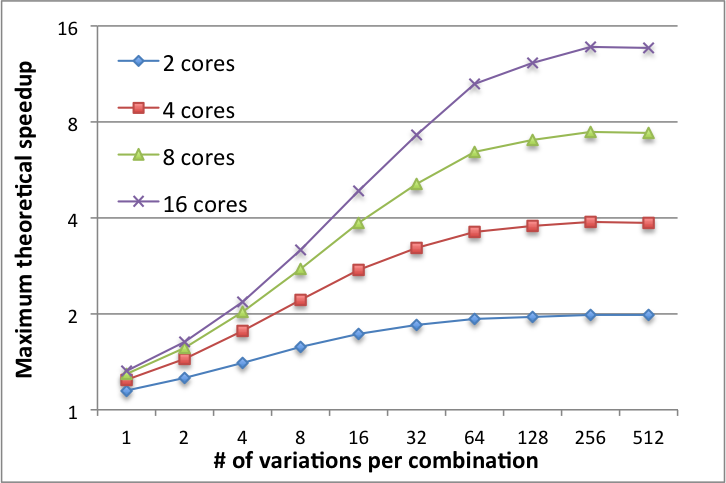
\includegraphics[scale=0.7]{../../common/graphs/amdahl_speedup.png}
		\caption{Theoretical speedup (Amdahl's Law) for various number of cores.}
		\label{fig:AmdahlSpeedup}
	\end{center}
\end{figure}

The maximum theoretical speedup calculation, presented in figure \ref{fig:AmdahlSpeedup}, is based on the Amdahl's Law \cite{AMDAHL} which states the maximum attainable speedup based on the number of processors and the percentage of the execution time spent on the parallelizable region of the code. The efficiency of the parallelization of an application can be measured by the distance of the speedup curve to the Amdahl's speedup curve. The Amdahl's Law was calculated for the original application with the initial optimizations to assess the efficiency of only the parallelization resource usage.

\begin{figure}[!htp]
	\begin{center}
		\raisebox{-0.5\height}{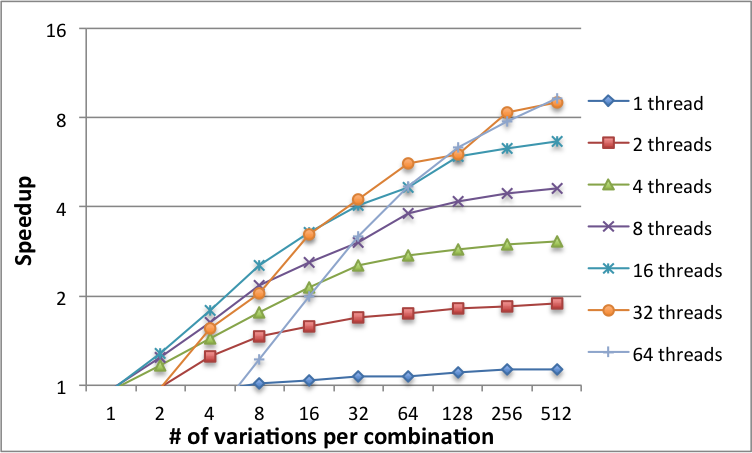
\includegraphics[scale=0.6]{../../common/graphs/speedup_nonpointer_static.png}}
		\raisebox{-0.5\height}{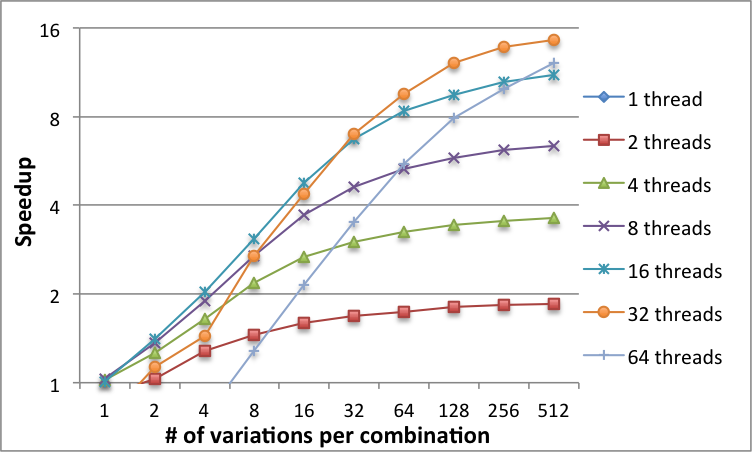
\includegraphics[scale=0.6]{../../common/graphs/speedup_nonpointer.png}}
		\caption{Speedup for the parallel non-pointer version of \tth application with static (left) and dynamic (right) scheduling.}
		\label{fig:RegularSpeedup}
	\end{center}
\end{figure}

Even with the performance increase provided by the optimizations in section \ref{InitialOptimizations}, for a low number of variations per combination the overhead of the thread management, data structure creation and best solution merge is too high and causes the application to be slower than the original. With the increase of threads, the thread management overhead increases and the performance is even lower. Overall, the best results are obtained using the dynamic scheduler. The dynamic scheduler overhead is evident when looking for the results using 1 thread, where the only overhead difference is only due to the schedulers: for 8 and more variations the static scheduler implementation offers speedups, while the dynamic scheduler implementation performance is always worse than the original application. Using all available cores (16 threads) offers a speedup of 6.7 and 9.2, for the static and dynamic scheduler versions respectively, in the best case of 512 variations. The use of hardware multithread (32 threads) benefits the performance in both cases, but the speedup is bigger for the dynamic scheduler implementation. It allows hiding the high latency of RAM memory acesses by scheduling threads which are ready to execute while others are idle waiting for the data. Multithreading managed by software (64 threads) offers speedups better than using 16 threads only high number of variations, such as 256 and 512. The best efficiency (speedups closest to the theoretical maximum) is obtained for 2, 4 and 32 threads of the dynamic scheduler implementation.

\begin{figure}[!htp]
	\begin{center}
		\raisebox{-0.5\height}{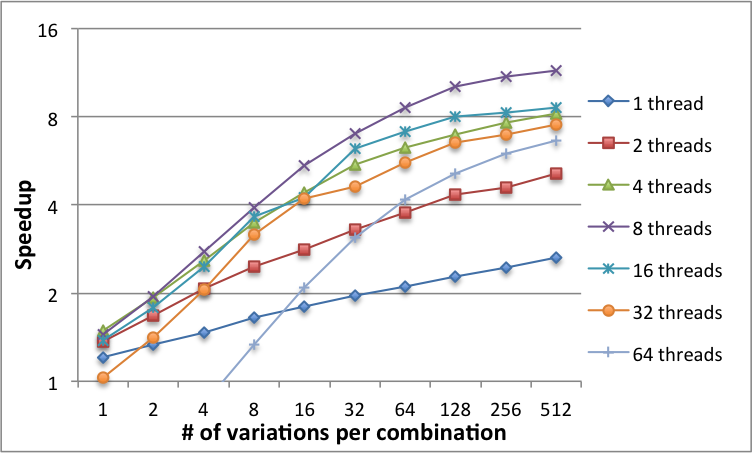
\includegraphics[scale=0.6]{../../common/graphs/speedup_pointer_static.png}}
		\raisebox{-0.5\height}{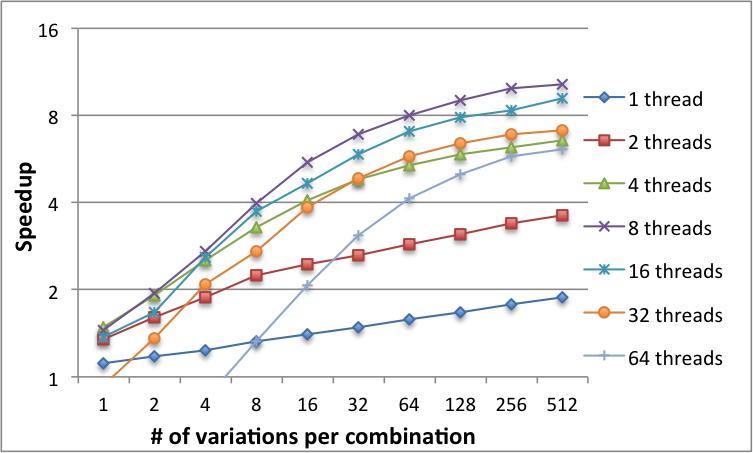
\includegraphics[scale=0.6]{../../common/graphs/speedup_pointer.png}}
		\caption{Speedup for the parallel pointer version of \tth application with static (left) and dynamic (right) scheduling.}
		\label{fig:PointerSpeedup}
	\end{center}
\end{figure}

Similar to the non-pointer version, the dynamic scheduling provides the best performance for high number of threads. However, for 2, 4 and 8 threads the low overhead of the static scheduler gives this implementation an advantage against the dynamic scheduler version. When both CPUs are used the performance of the static scheduler version degrades relatively to the dynamic scheduler. The difference between the overheads of the two schedulers is evident when comparing both implementations using only one thread. The most important result is the efficiency of the static scheduler implementation for 2, 4 and 8 threads, as they present superscalar speedup\footnote{Superscalar speedup occurs when the speedup is higher than the number of CPU cores used.}, mostly due to the pseudo-random number generation optimizations allied to the low overhead of constructing the data structure, as opposed to the higher overhead of the non-pointer version.

\begin{figure}[!htp]
	\begin{center}
		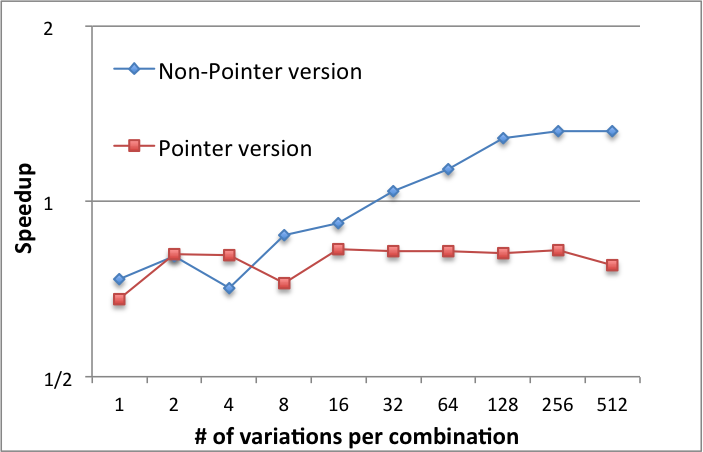
\includegraphics[scale=0.7]{../../common/graphs/ht_speedup.png}
		\caption{Theoretical speedup (Amdahl's Law) for various number of cores.}
		\label{fig:AmdahlSpeedup}
	\end{center}
\end{figure}

The speedup provided by the use of hardware multithreading, which helps to improve the CPU resource usage by scheduling by hardware two threads in each core, is only noticeable for 32 or more variations in the non-pointer implementation. It provides a speedup up to 1.3 over using only 1 thread per core, by diminishing the impact of high latency RAM memory accesses, as explained before. In the non-pointer implementation, hardware multithreading degrades performance due to the usage of pointers to shared memory, resulting in the increase of the latency of memory accesses proportional to the increase of threads used, as long as more than one CPU is used.

Considering only the dynamic scheduler non-pointer and the static scheduler pointer implementations, which present the best performance, the non-pointer version offers the best speedup for 32 threads. However, the best efficiency is obtained by the pointer version for 2, 4 and 8 threads, due to the reduced overhead of constructing the data structure, as explained in section \ref{SharedMemImplementation}. It provides a speedup of 11.5 for 8 threads and 512 variations, only matched by the non-pointer implementation using 16, 32 and 64 threads. For higher number of threads the performance does not increase, which is an expected behavior since threads in different CPUs share a pointer to the same data. The said data is only in one memory bank, forcing non-unified memory accesses that degrade the performance of the threads in one of the CPUs, and the data cannot be properly stored in the cache as the use of pointers prevents a vast set of memory management optimizations. Chosing the best implementation depends on the system, as the non-pointer version is best for multi-CPU systems while the pointer version is best for single CPU systems. VTune did not identify more possible bottlenecks and the optimization process stoped as the results are very close to the theoretical maximum.

\begin{figure}[!htp]
	\begin{center}
		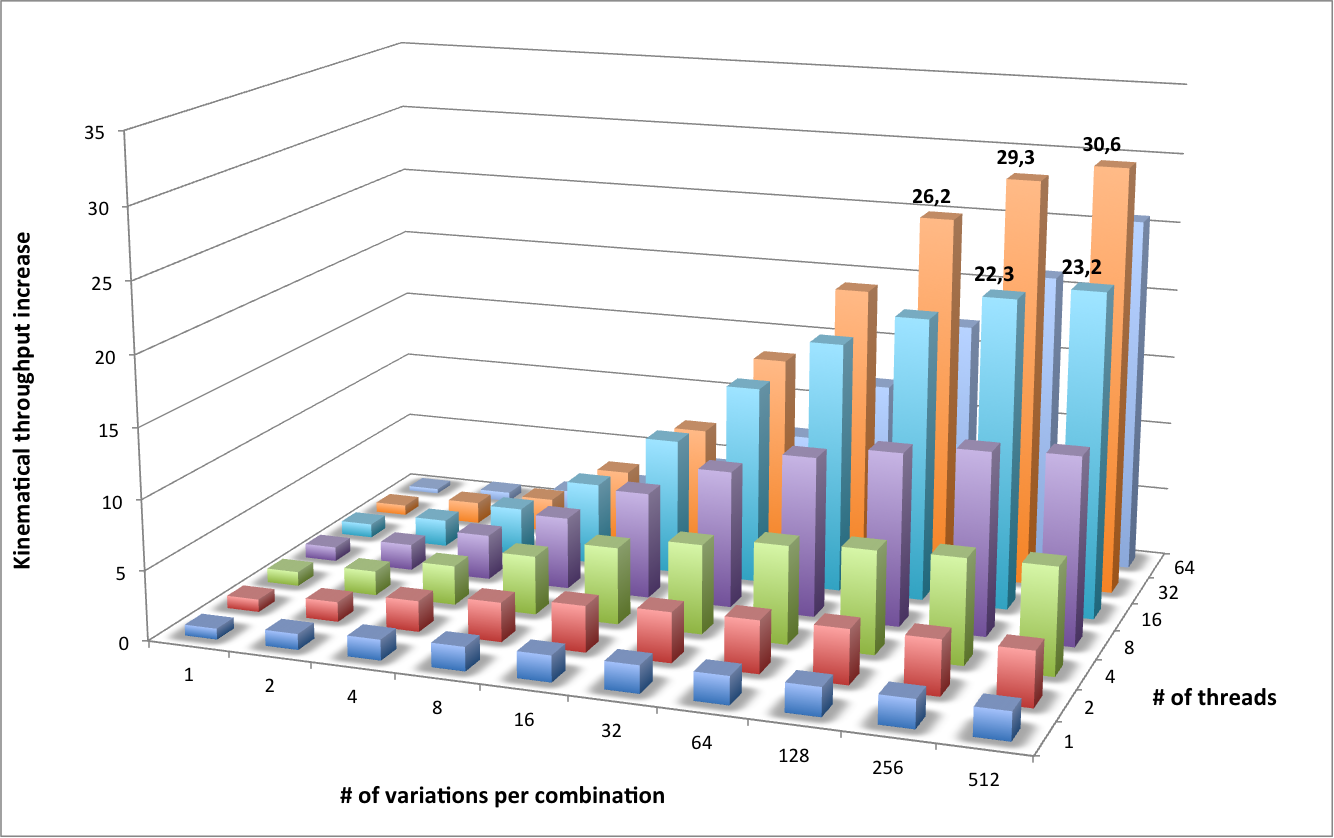
\includegraphics[scale=0.6]{../../common/graphs/dilep_throughput.png}
		\caption{Theoretical speedup (Amdahl's Law) for various number of cores.}
		\label{fig:DilepThroughput}
	\end{center}
\end{figure}

One possible metric to measure the increase of throughput in the \ttDilepKinFit is the increase of kinematical reconstructions performed relatively to the sequential application. Only this part of the function is suitable for this purpose as it is always executed for every variation of any combination, opposed to the Higgs Boson reconstruction which is only performed if the \ttbar system is reconstructed. The speedup of the kinematical reconstruction versus the original application is presented in figure \ref{fig:DilepThroughput}. The non-pointer implementation performs up to 30 times more kinematical reconstructions than the original application in the same time, for 512 variations and 32 threads. This value does not translate directly into overall application speedup at this only considers a regular task inside the bigger, irregular \ttDilepKinFit.

\begin{figure}[!htp]
	\begin{center}
		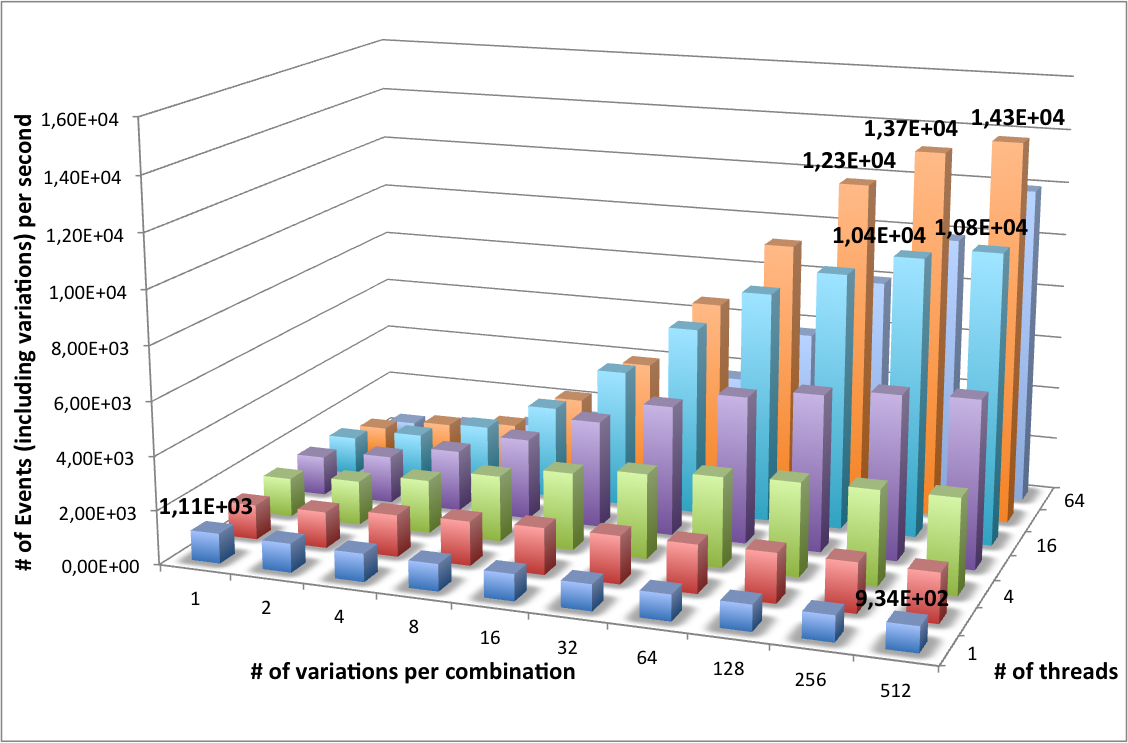
\includegraphics[scale=0.6]{../../common/graphs/throughput.png}
		\caption{Theoretical speedup (Amdahl's Law) for various number of cores.}
		\label{fig:EventThroughput}
	\end{center}
\end{figure}

One of the concerns for research groups is the amount of events that their applications are able to process. Figure \ref{fig:EventThroughput} presents the event throughput of the non-pointer implementation with the dynamic scheduler, with the purpose of identifying the maximum throughput possible due to parallelization. An event processing is considered to be all events in the input data file, as well as each individual variation reconstructions of those who reach cut number 20 of \tth. The sequential, already optimized, application is presented in the \"1 thread\" line on the graph. throughput is For 512 variations and 32 threads the event throughput is 14300 events per second, which is 15 times higher than the original for the same number of variations.

\todo{meter throughput da outra versao?}

\subsubsection{Performance analysis on various computational systems}
\label{SharedMemPerformanceVarious}

Scientific computer clusters are not always made of high end computing nodes, such as the compute-701 test system used. A simpler performance analysis on 3 dual-socket test systems common among research groups is presented in this subsection. Only the speedup and execution time will be compared, as an in-depth analysis was already made for the compute-701 system in section \ref{SharedMemPerformance}.

Only the two best implementations, non-pointer with dynamic scheduler and pointer with static scheduler, are tested for three different number of threads: one per core using one CPU; one per core using both CPUs; one per hardware thread if hardware multithreading is supported. The test systems used are the compute-401, compute-511 and compute-601 nodes of the SeARCH cluster\footnote{See appendix \ref{App:TestEnv} for the characterization of all test systems.}.

\begin{figure}[!htp]
	\begin{center}
		\raisebox{-0.5\height}{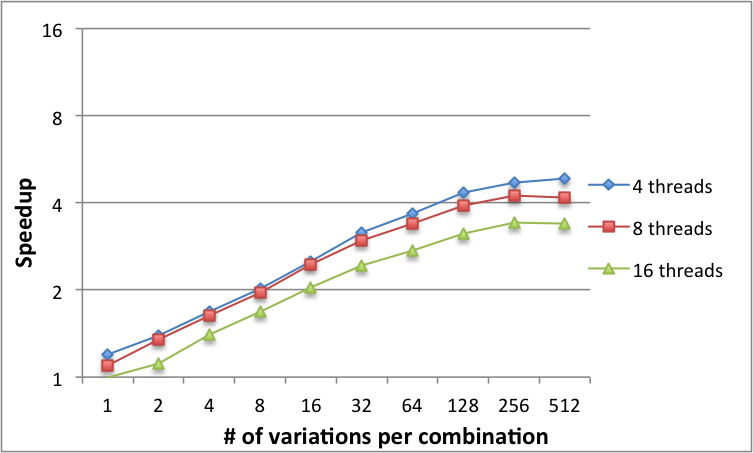
\includegraphics[scale=0.6]{../../common/graphs/speedup_pointer_401.png}}
		\raisebox{-0.5\height}{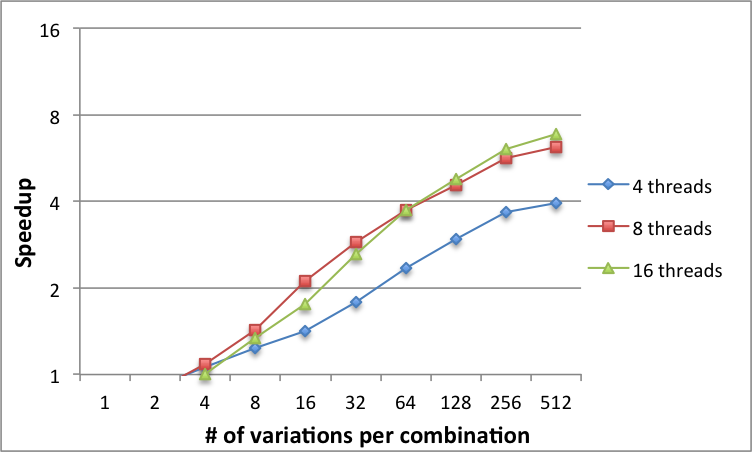
\includegraphics[scale=0.6]{../../common/graphs/speedup_nonpointer_401.png}}
		\caption{Speedup of the \tth application for pointer static (left) and non-pointer dynamic (right) scheduler implementations in the compute-401 node.}
		\label{fig:Speedup401}
	\end{center}
\end{figure}

\begin{figure}[!htp]
	\begin{center}
		\raisebox{-0.5\height}{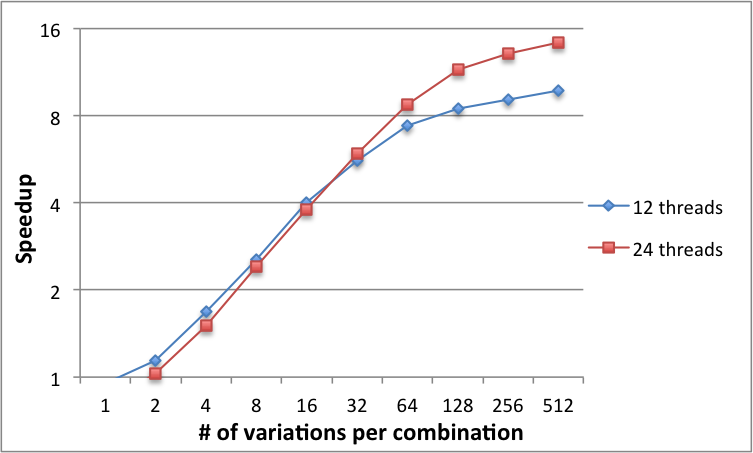
\includegraphics[scale=0.6]{../../common/graphs/speedup_pointer_511.png}}
		\raisebox{-0.5\height}{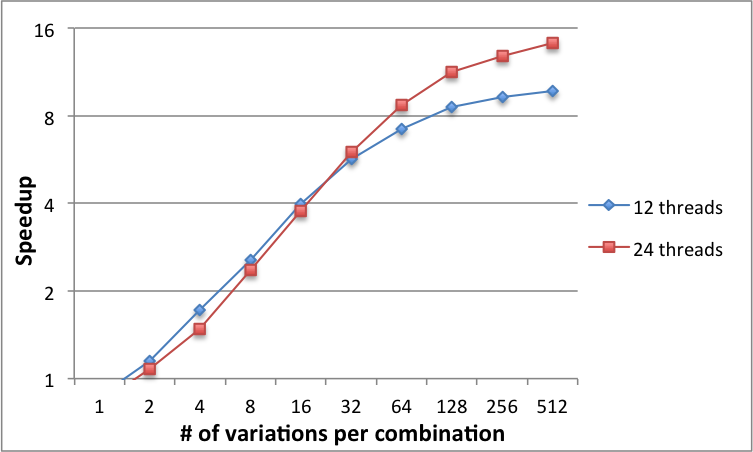
\includegraphics[scale=0.6]{../../common/graphs/speedup_nonpointer_511.png}}
		\caption{Speedup of the \tth application for pointer static (left) and non-pointer dynamic (right) scheduler implementations in the compute-511 node.}
		\label{fig:Speedup511}
	\end{center}
\end{figure}

\begin{figure}[!htp]
	\begin{center}
		\raisebox{-0.5\height}{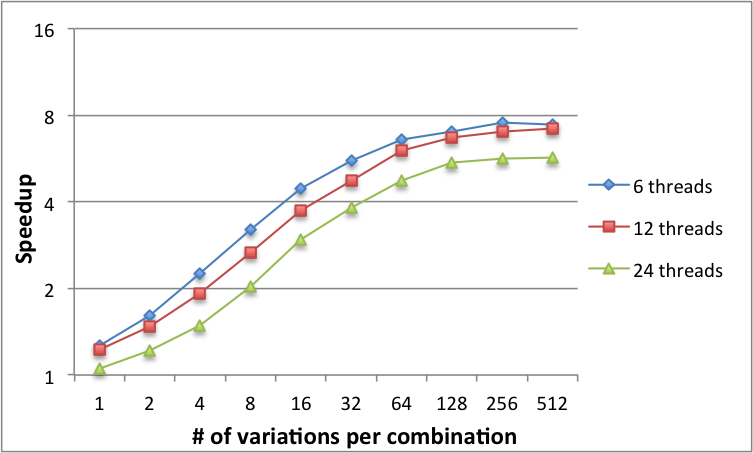
\includegraphics[scale=0.6]{../../common/graphs/speedup_pointer_601.png}}
		\raisebox{-0.5\height}{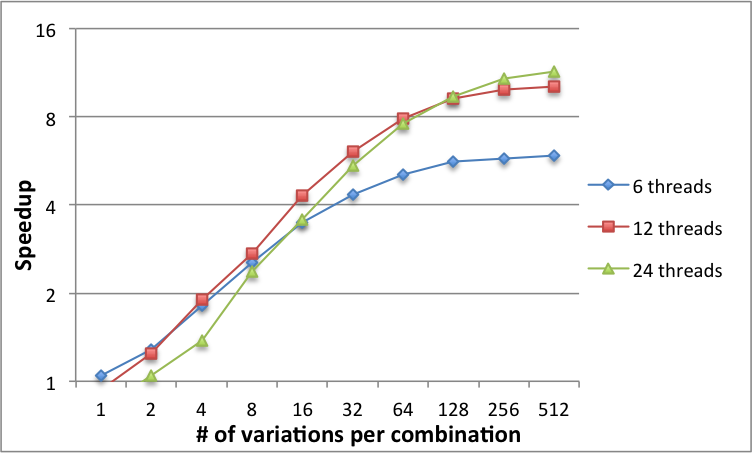
\includegraphics[scale=0.6]{../../common/graphs/speedup_nonpointer_601.png}}
		\caption{Speedup of the \tth application for pointer static (left) and non-pointer dynamic (right) scheduler implementations in the compute-601.}
		\label{fig:Speedup601}
	\end{center}
\end{figure}

\begin{figure}[!htp]
	\begin{center}
		\raisebox{-0.5\height}{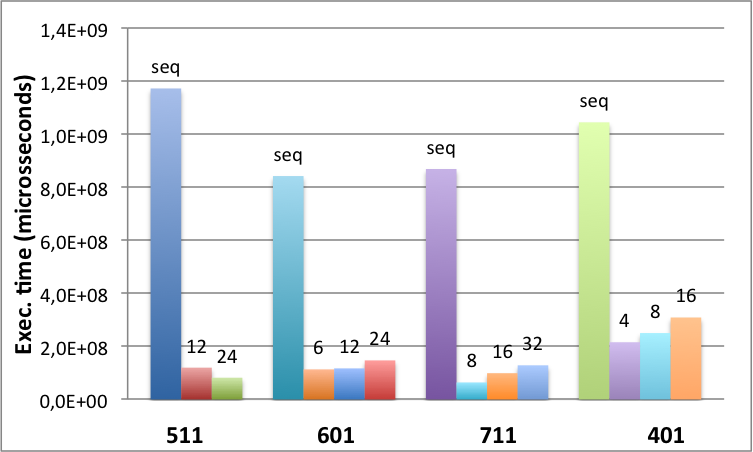
\includegraphics[scale=0.6]{../../common/graphs/exec_times_pointer.png}}
		\raisebox{-0.5\height}{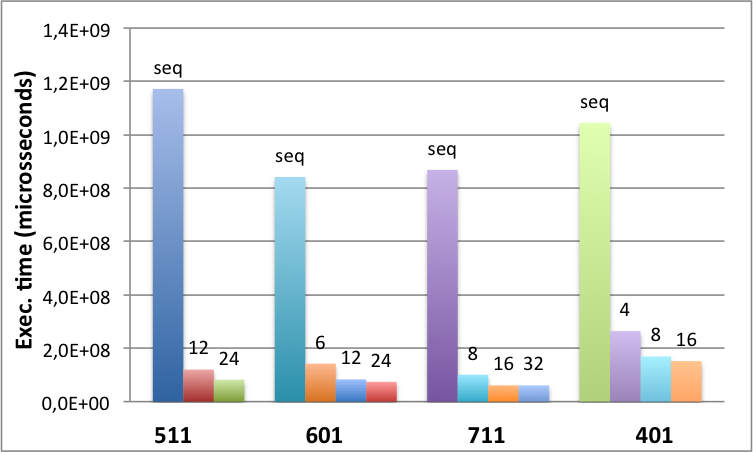
\includegraphics[scale=0.6]{../../common/graphs/exec_times_nonpointer.png}}
		\caption{Execution times of the \tth application for pointer static (left) and non-pointer dynamic (right) scheduler implementations.}
		\label{fig:ExecTimes}
	\end{center}
\end{figure}

\pdfbookmark{GPU Parallelization}{gpu parallelization}
\section{GPU Parallelization}
\label{Parallelization:GPU}

An early analysis of the code was made before designing the the workflow for the GPU parallelization. The implementation of this version will be restricted by the dependencies that \ttDilepKinFit has on ROOT classes, namely on its third stage of the generalist parallelizable workflow (figure \ref{fig:SeqPipeline}, right). It uses several functions and classes from ROOT, which can possibly be adapted to the GPU but the amount of time and work necessary to do so makes it unviable. The kinematic reconstruction also uses ROOT classes, namely TLorentzVectors, however it is read-only so it can be transformed in a data structure fit to be used on GPU. Note that this transformation will have a cost associated, which can slightly affect the performance.

\begin{figure}[!htp]
	\begin{center}
		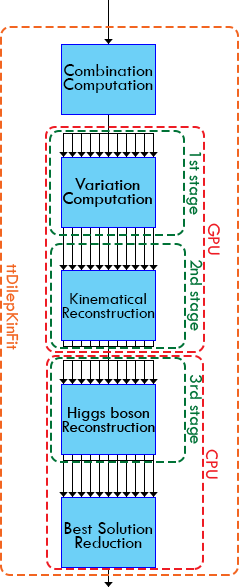
\includegraphics[scale=0.5]{../../common/img/gpu_pipeline.png}
		\caption{Schematic representation of the \ttDilepKinFit workflow.}
		\label{fig:GPUPipeline}
	\end{center}
\end{figure}

The first two stages of the the workflow presented in figure \ref{fig:SeqPipeline} (right), the computation of the variances and the kinematical reconstruction, can be adapted to run on the GPU. After computing the data structure holding the jets and leptons combinations, it must be transferred to the GPU (device) memory and then launch the kernel, where each task (which is refers to one combination) is assigned to one thread. The variation of the combinations is done by each thread, on the assigned combination, the kinematical reconstruction is computed and the results are transferred back to the CPU (host) memory. Then, the third stage of the workflow, the Higgs boson reconstruction, is performed on the host. Note that this process, copying the memory to the device and back to the host is done one time for each event processed. The schematic representation of the workflow for this implementation is presented in figure \ref{fig:GPUPipeline}.

This implementation has two factors which will restrict the performance. The first is the overhead associated to the transformation of the data (ROOT classes) to a suitable data structure to be used by the device. This happens with the input and output of the kernel. Even though this process can be tuned, which will be explained in section \ref{GPUImplementation}, there is no alternatives to study, algorithm-wise. The second factor is the synchronization and data transfer between host and device. The transfer time is affected by the amount of data to transfer, but it cannot be reduced since it is always necessary to transfer the jet/lepton combinations. Note that they are only transferred once per event, where the kernel threads copy the information so they can change it. However, the synchronization can be removed. The kernel can be launched and the threads are blocked while waiting for work, and then each time the one thread of the host computes a combination it is transferred to the device memory and the respective threads start the computation. Meanwhile, there is another thread in the host waiting for the results and starting the parallel computation of the Higgs boson reconstruction each time a group of kernel threads finish. If this asynchronous communication can be correctly implemented it might offer significant better performance than the synchronous version.

\section{MIC Parallelization}
\label{Parallelization:MIC}

\section{Scheduler Parallelization}
\label{Parallelization:Scheduler}
throughput scheduler
TESTES COM NOVO STATIC SCHEDULER NO POINTER